\section{Stejnoměrná spojitost}

\begin{definice}
  Řekneme, že fce $f_n(x) \colon I \to \mathbb R$ konvergují v $I$ bodově k funkci $f(x)\colon I \to \mathbb R$, jestliže
  $$\lim_{n \to \infty} f_n(x)\to f(x) \quad \forall x \in I \text{ pevné.}$$
  Značíme $f_n(x) \to f(x)$ v $I$.
\end{definice}

\begin{priklad}
  \begin{enumerate}[1)]
    \item $f_n(x) = (1+\frac{x}{n})^n \to e^x, x \in \mathbb R$; neboť $f_n(x) = e^{g_n(x)}$

    $g_n(x)=n\ln(1+\frac{x}{n})=\frac{\ln (1+\frac{x}{n})}{\frac{x}{n}}\cdot x\to x, n \to \infty, x \in \mathbb R, x \neq 0$ pevné

    $x=0\colon f_n(0) = (1+0)^n=1=e^0$
    \item $f_n(x)=\frac{nx}{1+n|x|} = \frac{x}{\frac{1}{n}+|x|} \left\{ \begin{array}{ll}
      \equiv 0 &x=0 \\ \to \frac{x}{0+|x|} &x \neq 0 \end{array} \right\} \sgn x, \forall x \in \mathbb R$

    \begin{figure}[ht!]
      \centering
      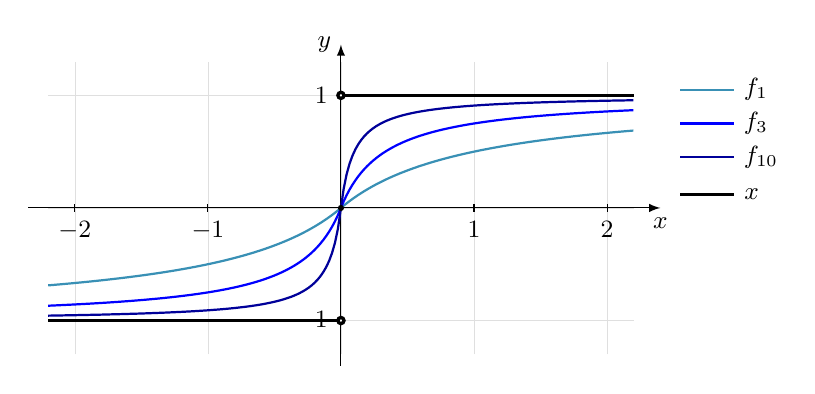
\begin{tikzpicture}[x=2.6cm, y=2.2cm, >=latex, font=\small, scale=0.65]

        \colorlet{fOne}{cyan!70!black}   % n = 1
        \colorlet{fThree}{blue}          % n = 3
        \colorlet{fTen}{blue!60!black}   % n = 10

  % grid and axes
  \draw[gray!25, very thin] (-2.2,-1.3) grid[step=1] (2.2,1.3);
  \draw[->] (-2.35,0) -- (2.4,0) node[below] {$x$};
  \draw[->] (0,-1.4) -- (0,1.45) node[left] {$y$};
  \foreach \x in {-2,-1,1,2}
    \draw (\x,2pt) -- (\x,-2pt) node[below] {$\x$};
  \foreach \y in {-1,1}
    \draw (2pt,\y) -- (-2pt,\y) node[left] {$\y$};

  % the sequence f_n (odd functions, so one plot covers both branches)
  \draw[fOne,   thick, domain=-2.2:2.2, samples=201]
    plot (\x, {\x/(1+abs(\x))});
  \draw[fThree, thick, domain=-2.2:2.2, samples=201]
    plot (\x, {3*\x/(1+3*abs(\x))});
  \draw[fTen,   thick, domain=-2.2:2.2, samples=201]
    plot (\x, {10*\x/(1+10*abs(\x))});

  % the limit: sgn x, drawn with sgn(0) = 0
  \draw[very thick] (-2.2,-1) -- (0,-1);
  \draw[very thick] (0,1)     -- (2.2,1);
  \draw[fill=white, very thick] (0,-1) circle[radius=1.7pt]; % jump not attained
  \draw[fill=white, very thick] (0,1)  circle[radius=1.7pt]; % jump not attained
  \fill (0,0) circle[radius=1.7pt];                          % sgn(0) = 0

  % legend
  \begin{scope}[every node/.style={font=\small}]
    \draw[fOne,   thick] (2.55,1.05) -- (2.95,1.05)
      node[right, black] {$f_1$};
    \draw[fThree, thick] (2.55,0.75) -- (2.95,0.75)
      node[right, black] {$f_3$};
    \draw[fTen,   thick] (2.55,0.45) -- (2.95,0.45)
      node[right, black] {$f_{10}$};
    \draw[very thick] (2.55,0.12) -- (2.95,0.12)
      node[right, black] {$\sgn x$};
  \end{scope}

\end{tikzpicture}
    \end{figure}

  \item $f_n(x)=n^2xe^{-nx} \to 0, \forall x \geq 0$

  \begin{figure}[ht!]
    \centering
    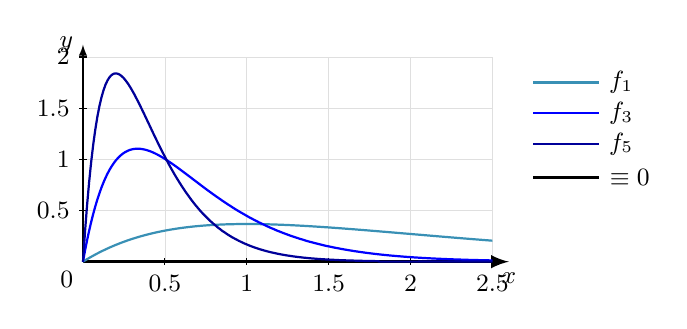
\begin{tikzpicture}[x=3.2cm, y=2cm, >=latex, font=\small, scale=0.65]

      \colorlet{fOne}{cyan!70!black}   % n = 1
\colorlet{fThree}{blue}          % n = 3
\colorlet{fFive}{blue!60!black}

  % grid
  \draw[gray!25, very thin] (0,0) grid[step=0.5] (2.5,2);

  % the limit f = 0 is the x-axis itself: draw it thick
  \draw[very thick, ->] (0,0) -- (2.6,0) node[below] {$x$};
  \draw[->] (0,0) -- (0,2.12) node[left] {$y$};
  \node[below left] at (0,0) {$0$};
  \foreach \x in {0.5,1,1.5,2,2.5}
    \draw (\x,2pt) -- (\x,-2pt) node[below] {$\x$};
  \foreach \y in {0.5,1,1.5,2}
    \draw (2pt,\y) -- (-2pt,\y) node[left] {$\y$};

  % the sequence f_n on x >= 0
  \draw[fOne,   thick, domain=0:2.5, samples=201] plot (\x, {\x*exp(-\x)});
  \draw[fThree, thick, domain=0:2.5, samples=201] plot (\x, {9*\x*exp(-3*\x)});
  \draw[fFive,  thick, domain=0:2.5, samples=201] plot (\x, {25*\x*exp(-5*\x)});

  % legend
  \begin{scope}[every node/.style={font=\small}]
    \draw[fOne,   thick] (2.75,1.75) -- (3.15,1.75)
      node[right, black] {$f_1$};
    \draw[fThree, thick] (2.75,1.45) -- (3.15,1.45)
      node[right, black] {$f_3$};
    \draw[fFive,  thick] (2.75,1.15) -- (3.15,1.15)
      node[right, black] {$f_5$};
    \draw[very thick] (2.75,0.82) -- (3.15,0.82)
      node[right, black] {$\equiv 0$};
  \end{scope}

\end{tikzpicture}
  \end{figure}
  \end{enumerate}
\end{priklad}

\begin{poznamka}
  Bodová konvergence má svá úskalí.
  \begin{itemize}
    \item $f_n(x)$ spojité, $f_n(x) \to f(x) \cancel{\implies} f(x)$ spojité
    \item $f_n(x) \to f(x)$ v $[a,b] \cancel{\implies} \int_a^b f_n \to \int_a^b f$
  \end{itemize}
  Zavedeme tedy silnější pojem.
\end{poznamka}

\begin{definice}
  Řekneme, že $f_n(x)$ konvergují stejnoměrně k $f(x)$ v $I$, jestliže
  $$(\forall \varepsilon > 0)(\exists n_0 \in \mathbb N)(\forall x \in I)[n\geq n_0 \implies |f_n(x)-f(x)|<\varepsilon].$$
  Značíme $f_n(x) \toto f(x)$ v $I$.

\begin{figure}[ht!]
    \centering

    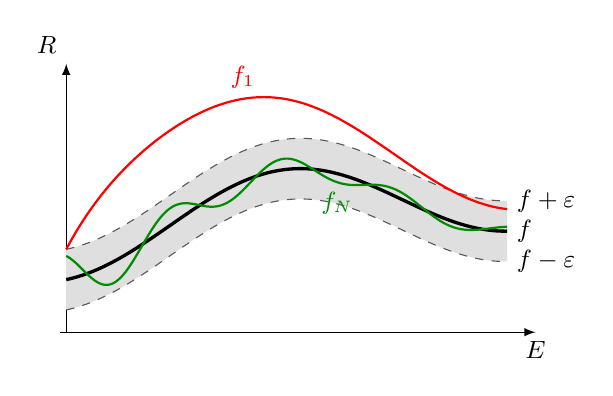
\begin{tikzpicture}[x=1.6cm, y=2.2cm, >=latex, font=\small, scale=0.5]

      % axes: domain E, values in R
      \draw[->] (0,-0.55) -- (0,2.55) node[above left] {$\mathbb{R}$};
      \draw[->] (-0.1,-0.55) -- (7.45,-0.55) node[below] {$E$};

      % shaded eps-tube between f+eps and f-eps
      \fill[gray!25]
        plot[domain=0:7, samples=120]
          (\x, {0.55 + 0.08*\x + 0.5*sin(deg(0.85*\x - 1.4)) + 0.35})
        -- plot[domain=7:0, samples=120]
          (\x, {0.55 + 0.08*\x + 0.5*sin(deg(0.85*\x - 1.4)) - 0.35})
        -- cycle;

      % dashed boundary curves of the tube
      \draw[gray!70!black, dashed, domain=0:7, samples=120]
        plot (\x, {0.55 + 0.08*\x + 0.5*sin(deg(0.85*\x - 1.4)) + 0.35});
      \draw[gray!70!black, dashed, domain=0:7, samples=120]
        plot (\x, {0.55 + 0.08*\x + 0.5*sin(deg(0.85*\x - 1.4)) - 0.35});
      \node[right, black] at (7,0.967) {$f+\varepsilon$};
      \node[right, black] at (7,0.267) {$f-\varepsilon$};

      % the limit function f
      \draw[black, very thick, domain=0:7, samples=200]
        plot (\x, {0.55 + 0.08*\x + 0.5*sin(deg(0.85*\x - 1.4))});
      \node[right] at (7,0.617) {$f$};

      % f_1 (red): starts near the tube, bulges out, returns for large x
      \draw[red, thick, domain=0:7, samples=200]
        plot (\x, {0.55 + 0.08*\x + 0.5*sin(deg(0.85*\x - 1.4))
                   + 1.3*\x*exp(-0.55*\x) + 0.35*exp(-0.25*\x)});
      \node[above, red] at (2.8,2.15) {$f_1$};

      % f_N (green): oscillates around f but stays inside the tube
      \draw[green!55!black, thick, domain=0:7, samples=200]
        plot (\x, {0.55 + 0.08*\x + 0.5*sin(deg(0.85*\x - 1.4))
                   + 0.3*exp(-0.25*\x)*sin(deg(3.5*\x + 2))});
      \node[below, green!55!black] at (4.3,1.18) {$f_N$};

    \end{tikzpicture}
\end{figure}
\end{definice}

\begin{poznamka}
  Přepisujme ekvivalentně definici bodové konvergence.

  $f_n(x) \to f(x), \forall x \in I$

  $(\forall x \in I)[\lim_{n\to \infty} f_n(x)=f(x)]$

  $(\forall x \in I)(\forall \varepsilon > 0)(\exists n_0 \in \mathbb N)[n\geq n_0 \implies |f_n(x)-f(x)|<\varepsilon]$

  $(\forall \varepsilon > 0)(\forall x \in I)(\exists n_0 \in \mathbb N)[n\geq n_0 \implies |f_n(x)-f(x)|<\varepsilon]$

  Rozdíl je v pořadí kvantifikace $x$ a $n_0$. Při bodové konvergenci nejprve fixuji $x$, pak volím $n_0$, tj. $n_0$ může obecně záviset na $x$. Při stejnoměrné konvergenci zvolené $n_0$ nezávisí na $x \in I$.
\end{poznamka}

\begin{veta}[Zachování spojitosti při stejnoměrné konvergenci]
  Nechť $f_n \in C(I)$, nechť $f_n \toto f$ v $I$. Pak $f \in C(I)$.
\end{veta}

\begin{proof}
  cíl: $(\forall x_0 \in I)(\forall \varepsilon > 0)(\exists \delta >0)[\underbrace{x \in \mathscr U(x_0, \delta)\cap I}_{|x-x_0|<\delta, x \in I}\implies \underbrace{f(x) \in \mathscr U(f(x_0),\varepsilon)}_{|f(x)-f(x_0)|<\varepsilon}]$

  OBRAZEKOBRAZEK

  $x_0 \in I, \varepsilon_0 >0$ libovolné, pevné

  víme: $f_n \toto f$ v $I$, a tedy $\exists n_0 \in \mathbb N$ t. ž. $|f(x)-f_{n_0}(x)|<\frac{\varepsilon}{3}, \forall x \in I \quad (+)$

  dále: $f_{n_0} \in C(I)$, a tedy $\exists \delta > 0$ t. ž. $x \in \mathscr U(x_0,\delta) \cap I \implies |f_{n_0}(x)-f_{n_0}(x_0)|<\frac{\varepsilon}{3} \quad (++)$

  \textsc{celkem}: $\forall x \in \mathscr U(x_0, \delta) \cap I\colon |f(x)-f(x_0)|=|f(x)-f_{n_0}(x)+f_{n_0}(x)-f_{n_0}(x_0)+f_{n_0}(x_0)-f(x_0)| \leq |f(x)-f_{n_0}(x)|+|f_{n_0}(x)-f_{n_0}(x_0)|+|f_{n_0}(x_0)-f(x_0)|<\footnotesize\underbrace{\frac{\varepsilon}{3}}_{(+)}+\underbrace{\frac{\varepsilon}{3}}_{(++)}+\underbrace{\frac{\varepsilon}{3}}_{(+)}=\varepsilon$
\end{proof}

\begin{veta}[Záměna limity a integrálu při stejnoměrné konvergenci]\label{16zamenalimint}
  Nechť $f_n \in C(I)$, nechť $f_n \toto f$ v $I$, kde $I=[a,b]$ je omezený a uzavřený. Pak
  $$\int_a^b f_n \to \int_a^b f, n \to \infty \quad \forall x \in I.$$
\end{veta}

\begin{proof}
  cíl: $\forall \varepsilon > 0 \; \exists n_0 \colon n \geq n_0 \implies |\int_a^b f_n - \int_a^b f|<\varepsilon$

  $\varepsilon > 0$ dáno, víme: $f_n \toto f$ v $[a, b]$, a tedy $\exists n_0 \in \mathbb N\colon |f_n(x)-f(x)|<\frac{\varepsilon}{b-a}, \forall x \in [a,b]$

  nechť $n \geq n_0\colon |\int_a^b f_n(x) \,\d x - \int_a^b f(x) \,\d x|=|\int_a^b(f_n(x)-f(x)) \,\d x| \leq \int_a^b (f_n(x)-f(x)) \,\d x < \frac{\varepsilon}{b-a}(b-a)=\varepsilon$
\end{proof}

\begin{poznamka}
  \begin{enumerate}
    \item $\lim_{n \to \infty}(\int_a^b f_n(x) \,\d x)\underbrace{=}_{\mathclap{\text{\uv{záměna} lim a } \int}}$
    \item Věta \ref{16zamenalimint} je \uv{příliš jednoduchá} (srovnej Leviho resp. Lebesgueova věta)
    \item Pro který integrál věta platí? Pro jakýkoliv!
  \end{enumerate}
\end{poznamka}

\begin{poznamka}
  Opakuj definici suprema (viz definice \ref{supremum}).
\end{poznamka}

\begin{lemma}
  Nechť $f_n(x), f(x)\colon I \to \mathbb R$. Pak je ekvivalentní
  \begin{enumerate}[1.]
    \item $f_n \toto f$ v $I$,
    \item $\sigma_n \to 0, n \to \infty$, kde $\sigma_n \coloneq \sup\limits_{x \in I}|f_n(x)-f(x)|$,
    \item $\forall$ posloupnosti $\{x_n\}\subset I$ platí, že $f_n(x_n) - f(x_n) \to 0, n \to \infty$.
  \end{enumerate}
\end{lemma}

\begin{proof}
  Dokážeme řetězec implikací.
  \begin{itemize}
    \item[$1. \implies 2.$] cíl: $\forall \varepsilon >0\; \exists n_0\colon n \geq n_0 \implies |\sigma_n| < \varepsilon$, tj. $\sigma_n < \varepsilon$, neboť $\sigma_n \geq 0$

    $\varepsilon >0$ dáno: díky $1.$ $\underbrace{\exists n_0\colon n \geq n_0 \implies |f_n(x)-f(x)|<\frac{\varepsilon}{2}}_{\textstyle \mathclap{\implies \sigma_n \underbrace{\leq}_{\textstyle \mathclap{\text{dle def. suprema}}} \frac{\varepsilon}{2}, \forall n \geq n_0 \implies \sigma_n < \varepsilon, \forall n \geq n_0}}, \forall x \in I$

    \item[$2. \implies 3.$] zřejmě platí $|f_n(x) -f(x)|\leq \sigma_n, \forall n \geq n_0, \forall x \in I$ dle definice suprema, a tedy pro libovolné $x_n \in I \colon |f_n(x_n)-f(x_n)|\leq \sigma_n, \forall n \geq n_0; \sigma_n \to 0$ dle $2.$, dále dle Věty TODO (VoDP)

    \item[$2. \implies 3.$] obměnou: $\neg 1. \implies \neg 3.$

    cíl: sestrojit $\{x_n\}$ t. ž. neplatí $3.$

    nechť $f_n \cancel{\toto} f$ v $I$, rozepišme

    $\neg (\forall \varepsilon > 0)(\exists n_0 \in \mathbb N)(\forall x \in I)[n \geq n_0 \implies |f_n(x)-f(x)|<\varepsilon]$, tj.

    $(\exists \varepsilon >0)(\forall n_0 \in \mathbb N)(\exists x \in I)(\exists n \geq n_0\colon |f_n(x)-f(x)|\geq \varepsilon)$

    $\varepsilon > 0$ fixuji, volím $n_0 = 1\colon \exists x = x_{k_1}, \exists n = k_1$ t. ž. $|f_{k_1}(x_k)-f(x_k)|\geq \varepsilon$

    indukcí: volím $n_0 = k_n + 1, \exists x = x_{k_{n+1}}, n = k_{n+1}$ t. ž. $|f_{k_n}(x_{k_n})-f(x_{k_n})|\geq \varepsilon$

    tj. máme podposloupnost indexů $k_1 < k_2 < \dots < k_n \to \infty$ t. ž. neplatí bod $3.$

    doplňme na posloupnost indexy $x_m \in I$, pro $m \notin \{k_n\}_{n=1}^{\infty}$ libovolně, a posloupnost stále nekonverguje do nuly (protože $\exists$ nekonvergující podposloupnost)
  \end{itemize}
\end{proof}

\begin{priklad}
  \begin{enumerate}[1.]
    \item $f_n(x) = \frac{nx}{1+n^2x^2}=f_1(nx)$, kde $f_1(x) = \frac{x}{1+x^2}$; $x \in [0, \infty)$

\begin{minipage}{0.58\textwidth}

    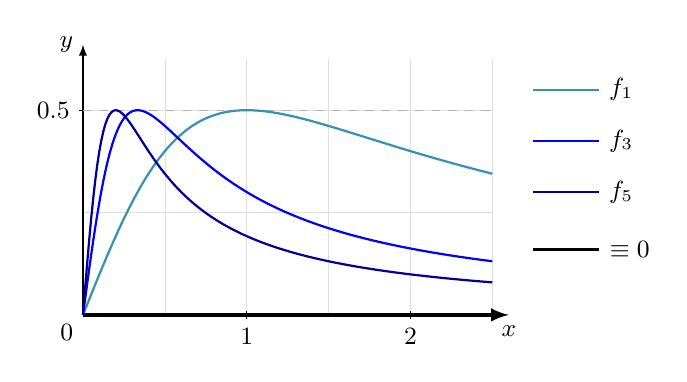
\begin{tikzpicture}[x=3.2cm, y=4cm, >=latex, font=\small, scale=0.65]

      \colorlet{fOne}{cyan!70!black}   % n = 1
      \colorlet{fThree}{blue}          % n = 3
      \colorlet{fFive}{blue!60!black}                % n = 5

  % grid
  \draw[gray!25, very thin] (0,0) grid[step=0.5] (2.5,1.25);

  % the limit f = 0 is the x-axis itself: draw it thick
  \draw[very thick, ->] (0,0) -- (2.6,0) node[below] {$x$};
  \draw[->] (0,0) -- (0,1.32) node[left] {$y$};
  \node[below left] at (0,0) {$0$};
  \foreach \x in {1,2}
    \draw (\x,2pt) -- (\x,-2pt) node[below] {$\x$};
  \foreach \y in {0.5}
    \draw (2pt,2*\y) -- (-2pt,2*\y) node[left] {$\y$};

  % peaks: max = 1/2 at x = 1/n -> add a dashed guide line at y = 1/2
  \draw[gray!60, dashed] (0,2*0.5) -- (2.5,2*0.5);

  % the sequence f_n on x >= 0
  \draw[fOne,   thick, domain=0:2.5, samples=201] plot (\x, {2*\x/(1+\x*\x)});
  \draw[fThree, thick, domain=0:2.5, samples=201] plot (\x, {2*3*\x/(1+9*\x*\x)});
  \draw[fFive,  thick, domain=0:2.5, samples=201] plot (\x, {2*5*\x/(1+25*\x*\x)});

  % legend
  \begin{scope}[every node/.style={font=\small}]
    \draw[fOne,   thick] (2.75,1.1) -- (3.15,1.1)
      node[right, black] {$f_1$};
    \draw[fThree, thick] (2.75,0.85) -- (3.15,0.85)
      node[right, black] {$f_3$};
    \draw[fFive,  thick] (2.75,0.6) -- (3.15,0.6)
      node[right, black] {$f_5$};
    \draw[very thick] (2.75,0.32) -- (3.15,0.32)
      node[right, black] {$\equiv 0$};
  \end{scope}

\end{tikzpicture}
\end{minipage}\begin{minipage}{0.42\textwidth}
$f_n(x) \to 0, n \to \infty, x \in I$ pevné

volme $x_n=\frac{1}{n}\in I$

$\left|f_n(x_n) - f(x_n)\right|=\left|\frac{n \frac{1}{n}}{1+\frac{n^2}{n^2}}-0\right|=\frac{1}{2} \cancel{\to} 0$

tj. $f_n \cancel{\toto} 0$ v $[0, \infty)$
\end{minipage}

A co $(0, \infty)$? Stejným argumentem $f_n \cancel{\toto} 0$ v $(0,\infty)$

A co $J=[\Delta, \infty), \Delta >0$ pevné?

\begin{minipage}{0.58\textwidth}
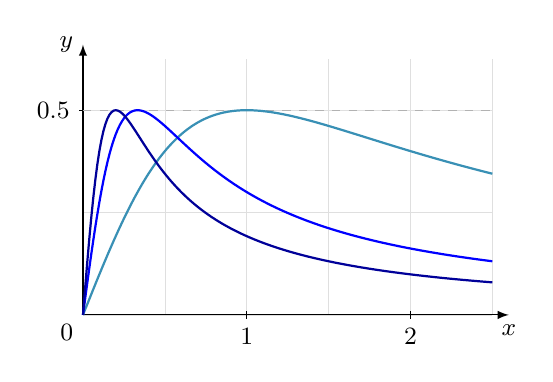
\begin{tikzpicture}[x=3.2cm, y=4cm, >=latex, font=\small, scale=0.65]

  \colorlet{fOne}{cyan!70!black}   % n = 1
  \colorlet{fThree}{blue}          % n = 3
  \colorlet{fFive}{blue!60!black}                % n = 5

% grid
\draw[gray!25, very thin] (0,0) grid[step=0.5] (2.5,1.25);

% the limit f = 0 is the x-axis itself: draw it thick
\draw[->] (0,0) -- (2.6,0) node[below] {$x$};
\draw[->] (0,0) -- (0,1.32) node[left] {$y$};
\node[below left] at (0,0) {$0$};
\foreach \x in {1,2}
\draw (\x,2pt) -- (\x,-2pt) node[below] {$\x$};
\foreach \y in {0.5}
\draw (2pt,2*\y) -- (-2pt,2*\y) node[left] {$\y$};

% peaks: max = 1/2 at x = 1/n -> add a dashed guide line at y = 1/2
\draw[gray!60, dashed] (0,2*0.5) -- (2.5,2*0.5);

% the sequence f_n on x >= 0
\draw[fOne,   thick, domain=0:2.5, samples=201] plot (\x, {2*\x/(1+\x*\x)});
\draw[fThree, thick, domain=0:2.5, samples=201] plot (\x, {2*3*\x/(1+9*\x*\x)});
\draw[fFive,  thick, domain=0:2.5, samples=201] plot (\x, {2*5*\x/(1+25*\x*\x)});


\end{tikzpicture}
\end{minipage}\begin{minipage}{0.42\textwidth}
$x_n = \frac{1}{n}<\Delta$ od jistého $n \geq n_0$

$\implies f_n$ klesá v $[\Delta, \infty]$, a tedy

$\sigma_n \coloneq \sup\limits{x \in J} \left|f_n(x)-f(x)\right|=f_n(\Delta) \to 0, n \to \infty$
\end{minipage}

tudíž $f_n \toto 0$ v $J$ dle věty \ref{16zamenalimint}, bod 2.
  \end{enumerate}
\end{priklad}

\begin{definice}
  Řekneme, že $f_n(x)$ konvergují lokálně stejnoměrně k $f(x)$ v $I$, jestliže
  $$(\forall x_0 \in I)(\exists \delta >0)[f_n \toto f \text{ v } \mathscr U(x_0, \delta) \cap I].$$
  Značíme $f_n \stackrel{\text{loc}}{\toto} f$ v $I$.
\end{definice}

\begin{priklad}
  $f_n(x)=\frac{nx}{1+n^2x^2} \stackrel{\text{loc}}{\toto} 0$ v $(0, \infty)$

  \begin{minipage}{0.58\textwidth}
  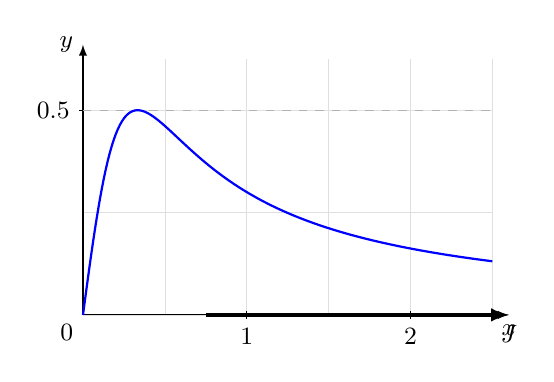
\begin{tikzpicture}[x=3.2cm, y=4cm, >=latex, font=\small, scale=0.65]

    \colorlet{fOne}{cyan!70!black}   % n = 1
    \colorlet{fThree}{blue}          % n = 3
    \colorlet{fFive}{blue!60!black}                % n = 5

  % grid
  \draw[gray!25, very thin] (0,0) grid[step=0.5] (2.5,1.25);

  % the limit f = 0 is the x-axis itself: draw it thick
  \draw[->] (0,0) -- (2.6,0) node[below] {$x$};
  \draw[very thick, ->] (0.75,0) -- (2.6,0) node[below] {$J$};
  \draw[->] (0,0) -- (0,1.32) node[left] {$y$};
  \node[below left] at (0,0) {$0$};
  \foreach \x in {1,2}
  \draw (\x,2pt) -- (\x,-2pt) node[below] {$\x$};
  \foreach \y in {0.5}
  \draw (2pt,2*\y) -- (-2pt,2*\y) node[left] {$\y$};

  % peaks: max = 1/2 at x = 1/n -> add a dashed guide line at y = 1/2
  \draw[gray!60, dashed] (0,2*0.5) -- (2.5,2*0.5);

  % the sequence f_n on x >= 0
  \draw[fThree, thick, domain=0:2.5, samples=201] plot (\x, {2*3*\x/(1+9*\x*\x)});

  \end{tikzpicture}
  \end{minipage}\begin{minipage}{0.42\textwidth}
  vezmu pro libovolné $x_0, \delta$ tak, aby bylo odražené od $0$, pak dle předchozího příkladu $\Delta, J$ TODO
  \end{minipage}
\end{priklad}

\begin{poznamka}
  \begin{itemize}
    \item $f_n \toto f$ v $J$, $\tilde{J} \subseteq J \implies f_n \toto f$ v $\tilde{J}$
    \item stejnoměrná konvergence $\implies$ lokální stejnoměrná konvergence $\implies$ bodová konvergence, žádnou implikaci nelze obrátit
  \end{itemize}
\end{poznamka}

\begin{poznamka}
  Opakuj definici Cauchyho-Bolzanovy podmínky pro posloupnosti a pro řady (definice \ref{7bc} a \ref{10bcr}) a věty o ekvivalenci B. C. podmínky a konvergence (věty \ref{7bckonv} a \ref{10bckonv}).
\end{poznamka}

\begin{definice}
  Řekneme, že posloupnost funkcí $\{f_n(x)\}_{n=1}^\infty$ splňuje Bolzanovu-Cauchyho podmínku stejnoměrné konvergence, jestliže
  $$(\forall \varepsilon >0)(\exists n_0 \in \mathbb N)(\forall x \in I)(\forall m,n \geq n_0)[|f_m(x)-f_n(x)|<\varepsilon]. \qquad \text{(B.C. st)}$$
\end{definice}

\begin{veta}
  Nechť $f_n(x)\colon I \to \mathbb R$ jsou dány. Pak je ekvivalentní
  \begin{enumerate}[1.]
    \item $\exists f(x)\colon I \to \mathbb R$ t. ž. $f_n(x) \toto f(x)$ v $I$,
    \item $\{f_n(x)\}$ splňuje (B.C. st)
  \end{enumerate}
\end{veta}

\begin{proof}
  TODO
\end{proof}

\begin{dusledek}
  $C_b(I)$ je úplný metrický prostor (fakticky i normovaný, tj. dokonce Banachův metrický prostor), kde $C_b(I) \coloneq \left\{f(x); f(x)\colon I \to \mathbb R\text{ spojité, omezené (b jako bounded)}\right\}$ a $\varrho(f,g) \coloneq \|f-g\|_\infty = \sup\limits_{x \in I} |f(x)-g(x)|$
\end{dusledek}

\begin{proof}
  TODO
\end{proof}

\begin{poznamka}
  \begin{itemize}
    \item $f_n \toto f$ v $I$ je ekvivalentní konvergenci vzhledem k $\|\cdot\|_\infty$, kde $\|f(x)\|_\infty = \sum\limits_{x \in I} |f(x)|$
    \item bodová (též slabá) konvergence nelze popsat ani normou, ani metrikou (pro $I$ nespočetné)
  \end{itemize}
\end{poznamka}

\begin{poznamka}
  Nechť $f_n(x) \colon (0, \infty) \to \mathbb R, n=1,2,\dots$ Pak
  $$\lim_{n\to \infty}\left(\lim_{x\to\infty}f_n(x)\right)\stackrel{?}{=}\lim_{x\to \infty}\left(\lim_{n\to\infty}f_n(x)\right)$$
  Obecně ne, ale někdy ano. Např. pro $f_n(x)=\arctg(\frac{x}{n})$ máme $\lim_{x\to \infty}\left(\lim_{n\to\infty}f_n(x)\right) = \frac{\pi}{2}$, ale $\lim_{n\to \infty}\left(\lim_{x\to\infty}f_n(x)\right) = 0$. Rovnost platí, pokud je alespoň jedna limita stejnoměrná.
\end{poznamka}
